% Source PDF page 181 (printed p. 167)
例如，$\alpha_2=-0.3$、$\gamma_1=0.5$ 意味着：化学物质1的浓度高于标称浓度时，年龄在1至2小时之间的细菌繁殖率下降，而年龄在0至1小时之间的细菌存活率上升。

假设可以通过给药，独立提高或降低浓度 $c_1,c_2$，例如在标称值的二倍范围内调整。问题是寻找使种群衰减最快，即使 $\lambda_{\mathrm{pf}}(A)$ 最小的药物组合。利用上述方法，可表述为GP
\[
\begin{array}{ll}
\text{最小化}&\lambda\\
\text{约束为}&b_1v_1+b_2v_2+b_3v_3+b_4v_4\le\lambda v_1,\\
&s_1v_1\le\lambda v_2,\\&s_2v_2\le\lambda v_3,\\&s_3v_3\le\lambda v_4,\\
&1/2\le c_i/c_i^{\mathrm{nom}}\le2,\quad i=1,2,\\
&b_i=b_i^{\mathrm{nom}}(c_1/c_1^{\mathrm{nom}})^{\alpha_i}(c_2/c_2^{\mathrm{nom}})^{\beta_i},\quad i=1,\ldots,4,\\
&s_i=s_i^{\mathrm{nom}}(c_1/c_1^{\mathrm{nom}})^{\gamma_i}(c_2/c_2^{\mathrm{nom}})^{\delta_i},\quad i=1,\ldots,3,
\end{array}
\]
变量为 $b_i,s_i,c_i,v_i,\lambda$。

\section{广义不等式约束}
标准形式凸优化问题（4.15）的一个很有用的推广，是允许不等式约束函数取向量值，并在约束中使用广义不等式：
\begin{equation}
\begin{array}{ll}\text{最小化}&f_0(x)\\\text{约束为}&f_i(x)\preceq_{K_i}0,\quad i=1,\ldots,m,\\&Ax=b,\end{array}\tag{4.48}
\end{equation}
其中 $f_0:\R^n\to\R$，$K_i\subseteq\R^{k_i}$ 为正常锥，$f_i:\R^n\to\R^{k_i}$ 为 $K_i$-凸函数。我们称其为具有广义不等式约束的标准形式凸优化问题。问题（4.15）是其中 $K_i=\R_+$（$i=1,\ldots,m$）的特例。

普通凸优化问题的许多结果对广义不等式问题仍然成立，例如：
\begin{itemize}
\item 可行集、任意下水平集和最优集均为凸集；
\item 问题（4.48）的任意局部最优点均为全局最优点；
\item §4.2.3给出的可微 $f_0$ 的最优性条件完全不变，仍然成立。
\end{itemize}
第11章还将看到，带广义不等式约束的凸优化问题通常可以像普通凸优化问题一样容易地求解。

% Source PDF page 182 (printed p. 168)
\subsection{锥形式问题}
带广义不等式的最简单凸优化问题之一，是锥形式问题，或称锥规划。其目标线性，只有一个不等式约束函数，并且该函数仿射，因而 $K$-凸：
\begin{equation}
\begin{array}{ll}\text{最小化}&c^\T x\\\text{约束为}&Fx+g\preceq_K0,\\&Ax=b.\end{array}\tag{4.49}
\end{equation}
当 $K$ 为非负正交象限时，锥形式问题退化为线性规划。因此，可将锥形式问题看作线性规划的推广，以广义线性不等式替换逐分量不等式。

继续类比线性规划，称
\[
\begin{array}{ll}\text{最小化}&c^\T x\\\text{约束为}&x\succeq_K0,\\&Ax=b\end{array}
\]
为标准形式的锥形式问题。类似地，称
\[
\begin{array}{ll}\text{最小化}&c^\T x\\\text{约束为}&Fx+g\preceq_K0\end{array}
\]
为不等式形式的锥形式问题。

\subsection{半正定规划}
当 $K$ 为 $k\times k$ 半正定矩阵构成的锥 $\mathbf S_+^k$ 时，相应锥形式问题称为半正定规划（SDP），形式为
\begin{equation}
\begin{array}{ll}\text{最小化}&c^\T x\\\text{约束为}&x_1F_1+\cdots+x_nF_n+G\preceq0,\\&Ax=b,\end{array}\tag{4.50}
\end{equation}
其中 $G,F_1,\ldots,F_n\in\mathbf S^k$，$A\in\R^{p\times n}$。这里的不等式是线性矩阵不等式，见例2.10。

若 $G,F_1,\ldots,F_n$ 全为对角矩阵，则（4.50）中的LMI等价于一组 $n$ 个线性不等式，SDP（4.50）就退化为线性规划。

\subsubsection*{标准形式与不等式形式的半正定规划}
类比LP，标准形式SDP具有线性等式约束，以及对变量 $X\in\mathbf S^n$ 的矩阵非负约束：
\begin{equation}
\begin{array}{ll}\text{最小化}&\tr(CX)\\\text{约束为}&\tr(A_iX)=b_i,\quad i=1,\ldots,p,\\&X\succeq0,\end{array}\tag{4.51}
\end{equation}

% Source PDF page 183 (printed p. 169)
其中 $C,A_1,\ldots,A_p\in\mathbf S^n$。（回顾 $\tr(CX)=\sum_{i,j=1}^n C_{ij}X_{ij}$ 是 $\mathbf S^n$ 上一般实值线性函数的形式。）可将它与标准形式线性规划（4.28）比较。在LP和SDP的标准形式中，都是在对变量施加 $p$ 个线性等式约束和一个非负约束的条件下，最小化变量的线性函数。

不等式形式SDP与不等式形式LP（4.29）对应，没有等式约束，只有一个LMI：
\[
\begin{array}{ll}\text{最小化}&c^\T x\\\text{约束为}&x_1A_1+\cdots+x_nA_n\preceq B,\end{array}
\]
变量为 $x\in\R^n$，参数为 $B,A_1,\ldots,A_n\in\mathbf S^k$、$c\in\R^n$。

\subsubsection*{多个LMI及线性不等式}
通常也将具有线性目标、线性等式与不等式约束，以及多个LMI约束的问题称为SDP，即
\[
\begin{array}{ll}
\text{最小化}&c^\T x\\
\text{约束为}&F^{(i)}(x)=x_1F_1^{(i)}+\cdots+x_nF_n^{(i)}+G^{(i)}\preceq0,\quad i=1,\ldots,K,\\
&Gx\preceq h,\quad Ax=b.
\end{array}
\]
将各个LMI和线性不等式组成一个大的块对角LMI，就容易变为SDP：
\[
\begin{array}{ll}\text{最小化}&c^\T x\\\text{约束为}&\diag(Gx-h,F^{(1)}(x),\ldots,F^{(K)}(x))\preceq0,\\&Ax=b.\end{array}
\]

\subsection{例子}
\subsubsection*{二阶锥规划}
SOCP（4.36）可表示为锥形式问题
\[
\begin{array}{ll}\text{最小化}&c^\T x\\\text{约束为}&-(A_ix+b_i,c_i^\T x+d_i)\preceq_{K_i}0,\quad i=1,\ldots,m,\\&Fx=g,\end{array}
\]
其中
\[
K_i=\{(y,t)\in\R^{n_i+1}\mid\norm{y}_2\le t\},
\]
即 $\R^{n_i+1}$ 的二阶锥。这就解释了优化问题（4.36）为何称为二阶锥规划。

\subsubsection*{矩阵范数最小化}
令 $A(x)=A_0+x_1A_1+\cdots+x_nA_n$，其中 $A_i\in\R^{p\times q}$。考虑无约束问题
\[
\text{最小化}\quad\norm{A(x)}_2,
\]

% Source PDF page 184 (printed p. 170)
其中 $\norm{\cdot}_2$ 为谱范数，即最大奇异值，变量为 $x\in\R^n$。由于 $\norm{A(x)}_2$ 是 $x$ 的凸函数，此问题是凸问题。

利用 $\norm{A}_2\le s$ 当且仅当 $A^\T A\preceq s^2I$ 且 $s\ge0$，可以将问题写为
\[
\begin{array}{ll}\text{最小化}&s\\\text{约束为}&A(x)^\T A(x)\preceq sI,\end{array}
\]
变量为 $x,s$。由于函数 $A(x)^\T A(x)-sI$ 关于 $(x,s)$ 矩阵凸，这是具有一个 $q\times q$ 矩阵不等式约束的凸优化问题。

也可以利用下述事实，将问题表述为具有一个 $(p+q)\times(p+q)$ 线性矩阵不等式的问题：
\[
A^\T A\preceq t^2I\text{ 且 }t\ge0
\quad\Longleftrightarrow\quad
\begin{bmatrix}tI&A\\A^\T&tI\end{bmatrix}\succeq0
\]
（见§A.5.5）。这得到以 $x,t$ 为变量的SDP
\[
\begin{array}{ll}\text{最小化}&t\\\text{约束为}&\begin{bmatrix}tI&A(x)\\A(x)^\T&tI\end{bmatrix}\succeq0.\end{array}
\]

\subsubsection*{矩问题}
设 $t$ 是 $\R$ 上的随机变量。期望 $\E t^k$（若存在）称为 $t$ 的分布的幂矩。以下经典结果刻画了矩序列。

若存在 $\R$ 上的概率分布，使 $x_k=\E t^k$（$k=0,\ldots,2n$），则 $x_0=1$，并且
\begin{equation}
H(x_0,\ldots,x_{2n})=
\begin{bmatrix}
x_0&x_1&x_2&\cdots&x_{n-1}&x_n\\
x_1&x_2&x_3&\cdots&x_n&x_{n+1}\\
x_2&x_3&x_4&\cdots&x_{n+1}&x_{n+2}\\
\vdots&\vdots&\vdots&&\vdots&\vdots\\
x_{n-1}&x_n&x_{n+1}&\cdots&x_{2n-2}&x_{2n-1}\\
x_n&x_{n+1}&x_{n+2}&\cdots&x_{2n-1}&x_{2n}
\end{bmatrix}\succeq0.\tag{4.52}
\end{equation}
矩阵 $H$ 称为与 $x_0,\ldots,x_{2n}$ 对应的Hankel矩阵。证明很简单：设 $x_i=\E t^i$（$i=0,\ldots,2n$）为某个分布的矩，$y=(y_0,y_1,\ldots,y_n)\in\R^{n+1}$，则
\[
y^\T H(x_0,\ldots,x_{2n})y
=\sum_{i,j=0}^n y_iy_j\E t^{i+j}
=\E(y_0+y_1t^1+\cdots+y_nt^n)^2\ge0.
\]
以下部分逆命题则不那么显然：若 $x_0=1$ 且 $H(x)\succ0$，则存在 $\R$ 上的概率分布，使 $x_i=\E t^i$（$i=0,\ldots,2n$）。

% Source PDF page 185 (printed p. 171)
证明见习题2.37。现在假设 $x_0=1$、$H(x)\succeq0$，但可能 $H(x)\not\succ0$，即线性矩阵不等式（4.52）成立，但未必严格成立。此时存在 $\R$ 上的一列分布，其矩收敛到 $x$。综上，$x_0,\ldots,x_{2n}$ 是某个 $\R$ 上分布的矩，或是一列分布的矩的极限，这一条件可表示为变量 $x$ 的LMI（4.52），加上线性等式 $x_0=1$。由此可将一些有趣的矩问题表述为SDP。

设 $t$ 为 $\R$ 上的随机变量。虽然不知道它的分布，但知道一些矩的界，即
\[
\underline\mu_k\le\E t^k\le\overline\mu_k,\quad k=1,\ldots,2n,
\]
这包括知道某些矩的精确值这一特例。给定 $t$ 的多项式 $p(t)=c_0+c_1t+\cdots+c_{2n}t^{2n}$，其期望关于各阶矩线性：
\[
\E p(t)=\sum_{i=0}^{2n}c_i\E t^i=\sum_{i=0}^{2n}c_ix_i.
\]
为计算满足给定矩界的全部概率分布中 $\E p(t)$ 的上下界，
\[
\begin{array}{ll}\text{最小化（最大化）}&\E p(t)\\\text{约束为}&\underline\mu_k\le\E t^k\le\overline\mu_k,\quad k=1,\ldots,2n,\end{array}
\]
可以求解SDP
\[
\begin{array}{ll}\text{最小化（最大化）}&c_1x_1+\cdots+c_{2n}x_{2n}\\\text{约束为}&\underline\mu_k\le x_k\le\overline\mu_k,\quad k=1,\ldots,2n,\\&H(1,x_1,\ldots,x_{2n})\succeq0,\end{array}
\]
变量为 $x_1,\ldots,x_{2n}$。这给出全部满足已知矩约束的分布中 $\E p(t)$ 的界。此界是紧的，含义是：存在一列分布，其矩满足给定的矩界，而 $\E p(t)$ 收敛到这些SDP求得的上下界。

\subsubsection*{协方差信息不完整时投资组合风险的界}
再次考虑经典Markowitz投资组合问题的设置，见第155页。有 $n$ 种资产或股票，$x_i$ 表示某一投资时期持有的资产 $i$ 的数量，$p_i$ 表示这一时期内资产 $i$ 的相对价格变化。组合总价值变化为 $p^\T x$。价格变化向量 $p$ 建模为随机向量，均值与协方差为
\[
\bar p=\E p,\qquad\Sigma=\E(p-\bar p)(p-\bar p)^\T.
\]
因此，组合价值变化为随机变量，均值 $\bar p^\T x$、标准差 $\sigma=(x^\T\Sigma x)^{1/2}$。较大损失的风险，即组合价值变化显著低于期望的风险，与标准差 $\sigma$ 直接相关，并随其增大而上升。

% Source PDF page 186 (printed p. 172)
因此，用标准差 $\sigma$ 或方差 $\sigma^2$ 衡量投资组合风险。

经典投资组合优化中，投资组合 $x$ 是变量，在最低平均收益和其他约束下最小化风险；价格变化统计量 $\bar p,\Sigma$ 为已知参数。这里的风险界问题反过来考虑：假设组合 $x$ 已知，但只知道协方差矩阵 $\Sigma$ 的部分信息。例如，知道每个元素的上下界
\[
L_{ij}\le\Sigma_{ij}\le U_{ij},\quad i,j=1,\ldots,n,
\]
其中 $L,U$ 给定。我们要问：在全部与给定界相容的协方差矩阵中，组合的最大风险是多少？定义组合的最坏情形方差为
\[
\sigma_{\mathrm{wc}}^2=\sup\{x^\T\Sigma x\mid L_{ij}\le\Sigma_{ij}\le U_{ij},\ i,j=1,\ldots,n,\ \Sigma\succeq0\}.
\]
这里加入了协方差矩阵当然必须满足的条件 $\Sigma\succeq0$。

可以通过求解SDP
\[
\begin{array}{ll}\text{最大化}&x^\T\Sigma x\\\text{约束为}&L_{ij}\le\Sigma_{ij}\le U_{ij},\quad i,j=1,\ldots,n,\\&\Sigma\succeq0\end{array}
\]
求出 $\sigma_{\mathrm{wc}}$，变量为 $\Sigma\in\mathbf S^n$，参数为 $x,L,U$。最优 $\Sigma$ 是满足元素界的最坏协方差矩阵，这里“最坏”指给定组合 $x$ 下的风险最大。由SDP的最优 $\Sigma$ 很容易构造一个满足给定界且达到最坏情形方差的 $p$ 的分布。例如，取 $p=\bar p+\Sigma^{1/2}v$，其中 $v$ 为任意满足 $\E v=0$、$\E vv^\T=I$ 的随机向量。

显然，对关于 $\Sigma$ 的任意凸先验信息，都可用同样方法确定 $\sigma_{\mathrm{wc}}$。下面列举若干例子。
\begin{itemize}
\item \textbf{某些投资组合的方差已知。}可以有形如
\[
u_k^\T\Sigma u_k=\sigma_k^2
\]
的等式约束，其中 $u_k,\sigma_k$ 已知。这对应知道某些已知组合 $u_k$ 的方差，或能非常准确地估计其方差。
\item \textbf{计入估计误差的影响。}若协方差 $\Sigma$ 从经验数据估计，估计方法会给出估计值 $\widehat\Sigma$，以及置信椭球等反映可靠性的信息。可将其表示为
\[
C(\Sigma-\widehat\Sigma)\le\alpha,
\]
其中 $C$ 是 $\mathbf S^n$ 上的正定二次型，常数 $\alpha$ 决定置信水平。
% Source PDF page 187 (printed p. 173)
\item \textbf{因子模型。}协方差可能形如
\[
\Sigma=F\Sigma_{\mathrm{factor}}F^\T+D,
\]
其中 $F\in\R^{n\times k}$、$\Sigma_{\mathrm{factor}}\in\mathbf S^k$，$D$ 为对角矩阵。这对应价格变化模型
\[
p=Fz+d,
\]
其中 $z$ 为随机变量，表示影响价格变化的底层因子，而 $d_i$ 相互独立，表示各资产价格的额外波动。假设因子已知。由于 $\Sigma$ 与 $\Sigma_{\mathrm{factor}},D$ 之间具有线性关系，可对后两者施加任意反映先验信息的凸约束，仍能用凸优化计算 $\sigma_{\mathrm{wc}}$。
\item \textbf{相关系数信息。}最简单的情形是 $\Sigma$ 的对角元素已知，即各资产价格波动程度已知，并且知道价格变化之间相关系数的界：
\[
l_{ij}\le\rho_{ij}=\frac{\Sigma_{ij}}{\Sigma_{ii}^{1/2}\Sigma_{jj}^{1/2}}\le u_{ij},\quad i,j=1,\ldots,n.
\]
由于 $\Sigma_{ii}$ 已知，而 $i\ne j$ 时的 $\Sigma_{ij}$ 未知，这些是线性不等式。
\end{itemize}

\subsubsection*{图上混合最快的马尔可夫链}
考虑无向图，结点为 $1,\ldots,n$，边集为
\[
\mathcal E\subseteq\{1,\ldots,n\}\times\{1,\ldots,n\}.
\]
$(i,j)\in\mathcal E$ 表示结点 $i,j$ 间有边。由于图无向，$\mathcal E$ 对称，即 $(i,j)\in\mathcal E$ 当且仅当 $(j,i)\in\mathcal E$。允许自环，即可以有 $(i,i)\in\mathcal E$。

定义马尔可夫链，状态为 $X(t)\in\{1,\ldots,n\}$，其中 $t\in\Z_+$，即非负整数。为每条边 $(i,j)\in\mathcal E$ 关联概率 $P_{ij}$，表示 $X$ 在结点 $i,j$ 之间转移的概率。状态只能沿边转移，故 $(i,j)\notin\mathcal E$ 时 $P_{ij}=0$。各边概率非负；对每个结点，与之相连的边的概率之和必须为一，包括存在的自环。

马尔可夫链的转移概率矩阵为
\[
P_{ij}=\Prob(X(t+1)=i\mid X(t)=j),\quad i,j=1,\ldots,n.
\]
矩阵必须满足
\begin{equation}
P_{ij}\ge0,\quad i,j=1,\ldots,n,\qquad\one^\T P=\one^\T,\qquad P=P^\T,\tag{4.53}
\end{equation}
以及
\begin{equation}
P_{ij}=0\quad\text{若 }(i,j)\notin\mathcal E.\tag{4.54}
\end{equation}

% Source PDF page 188 (printed p. 174)
由于 $P$ 对称且 $\one^\T P=\one^\T$，可得 $P\one=\one$，所以均匀分布 $(1/n)\one$ 是此链的平衡分布。$X(t)$ 的分布收敛到 $(1/n)\one$ 的速度由 $P$ 按模排列第二大的特征值决定，即由 $r=\max\{\lambda_2,-\lambda_n\}$ 决定，其中
\[
1=\lambda_1\ge\lambda_2\ge\cdots\ge\lambda_n
\]
为 $P$ 的特征值。称 $r$ 为马尔可夫链的混合率。

若 $r=1$，$X(t)$ 的分布未必收敛到 $(1/n)\one$，即马尔可夫链不混合。当 $r<1$ 时，$t\to\infty$ 时 $X(t)$ 的分布按 $r^t$ 渐近接近 $(1/n)\one$。所以 $r$ 越小，马尔可夫链混合越快。

最快混合马尔可夫链问题，是在约束（4.53）、（4.54）下寻找使 $r$ 最小的 $P$。（问题数据是图，即边集 $\mathcal E$。）下面说明它可表述为SDP。

特征值 $\lambda_1=1$ 对应特征向量 $\one$，所以混合率可表示为 $P$ 在子空间 $\one^\perp$ 上的限制的范数：$r=\norm{QPQ}_2$，其中 $Q=I-(1/n)\one\one^\T$ 表示到 $\one^\perp$ 的正交投影。利用 $P\one=\one$，有
\[
\begin{aligned}
r&=\norm{QPQ}_2\\
&=\norm{(I-(1/n)\one\one^\T)P(I-(1/n)\one\one^\T)}_2\\
&=\norm{P-(1/n)\one\one^\T}_2.
\end{aligned}
\]
这说明混合率 $r$ 为 $P$ 的凸函数，所以最快混合马尔可夫链问题可写成凸优化问题
\[
\begin{array}{ll}\text{最小化}&\norm{P-(1/n)\one\one^\T}_2\\\text{约束为}&P\one=\one,\\&P_{ij}\ge0,\quad i,j=1,\ldots,n,\\&P_{ij}=0\quad\text{若 }(i,j)\notin\mathcal E,\end{array}
\]
变量为 $P\in\mathbf S^n$。引入标量变量 $t$ 对 $P-(1/n)\one\one^\T$ 的范数给出上界，即可表示为SDP：
\begin{equation}
\begin{array}{ll}\text{最小化}&t\\\text{约束为}&-tI\preceq P-(1/n)\one\one^\T\preceq tI,\\&P\one=\one,\\&P_{ij}\ge0,\quad i,j=1,\ldots,n,\\&P_{ij}=0\quad\text{若 }(i,j)\notin\mathcal E.\end{array}\tag{4.55}
\end{equation}

\section{向量优化}
\subsection{一般向量优化问题与凸向量优化问题}
§4.6将标准形式问题（4.1）推广到向量值约束函数。本节研究向量值目标函数的含义。

% Source PDF page 189 (printed p. 175)
一般向量优化问题记为
\begin{equation}
\begin{array}{ll}\text{最小化（关于 }K\text{）}&f_0(x)\\\text{约束为}&f_i(x)\le0,\quad i=1,\ldots,m,\\&h_i(x)=0,\quad i=1,\ldots,p.\end{array}\tag{4.56}
\end{equation}
这里 $x\in\R^n$ 为优化变量，$K\subseteq\R^q$ 为正常锥，$f_0:\R^n\to\R^q$ 为目标函数，$f_i:\R^n\to\R$ 为不等式约束函数，$h_i:\R^n\to\R$ 为等式约束函数。它与标准优化问题（4.1）的唯一区别在于：这里目标取 $\R^q$ 中的值，问题还指定了用于比较目标值的正常锥 $K$。在向量优化的语境下，有时称标准优化问题（4.1）为标量优化问题。

若目标 $f_0$ 为 $K$-凸函数，不等式约束函数 $f_1,\ldots,f_m$ 凸，等式约束函数 $h_1,\ldots,h_p$ 仿射，就称（4.56）为凸向量优化问题。（和标量情形一样，通常将等式约束写为 $Ax=b$，其中 $A\in\R^{p\times n}$。）

怎样理解向量优化问题（4.56）？设 $x,y$ 为两个可行点，即满足全部约束。对应目标值 $f_0(x),f_0(y)$ 要通过广义不等式 $\preceq_K$ 比较。$f_0(x)\preceq_K f_0(y)$ 表示：以目标 $f_0$ 关于 $K$ 衡量时，$x$ 的价值“优于或等于”$y$。向量优化令人困惑之处是，两个目标值 $f_0(x),f_0(y)$ 未必可比；可能既没有 $f_0(x)\preceq_K f_0(y)$，也没有 $f_0(y)\preceq_K f_0(x)$，即谁也不比谁好。标量目标优化中不会出现这种情形。

\subsection{最优点与最优值}
先考虑向量优化问题含义明确的一种特殊情形。可行点的目标值集合
\[
\mathcal O=\{f_0(x)\mid\exists x\in\mathcal D,\ f_i(x)\le0,\ i=1,\ldots,m,\ h_i(x)=0,\ i=1,\ldots,p\}\subseteq\R^q
\]
称为可达目标值集。若该集合有最小元（见§2.4.2），即存在可行点 $x$，使对所有可行点 $y$ 有 $f_0(x)\preceq_K f_0(y)$，就称 $x$ 为问题（4.56）的最优点，称 $f_0(x)$ 为最优值。（向量优化问题若有最优值，则它唯一。）若 $x^\star$ 最优，$f_0(x^\star)$ 就可与其他每个可行点的目标值比较，且优于或等于它。粗略地说，$x^\star$ 是可行点中一个无歧义的最佳选择。

点 $x^\star$ 最优，当且仅当它可行且
\begin{equation}
\mathcal O\subseteq f_0(x^\star)+K\tag{4.57}
\end{equation}

% Source PDF page 190 (printed p. 176)
\begin{figure}[htbp]
\centering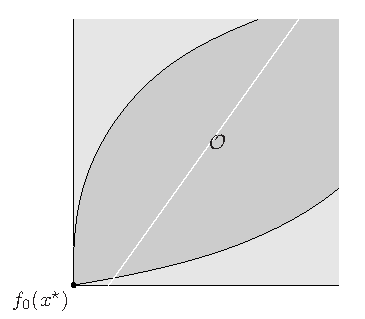
\includegraphics[width=.60\textwidth]{figures/ch04-07.pdf}
\caption*{图4.7\quad 向量优化的可达值集 $\mathcal O$ 为阴影部分，目标值位于 $\R^2$，锥为 $K=\R_+^2$。此时标出的 $f_0(x^\star)$ 是问题的最优值，$x^\star$ 为最优点。目标值 $f_0(x^\star)$ 可与每个其他可达值 $f_0(y)$ 比较，且优于或等于 $f_0(y)$。（这里“优于或等于”指“位于下方和左方”。）浅阴影区域为 $f_0(x^\star)+K$，即对应于比 $f_0(x^\star)$ 更差或与之相等的目标值的所有 $z\in\R^2$ 的集合。}
\end{figure}
（见§2.4.2）。集合 $f_0(x^\star)+K$ 可解释为比 $f_0(x^\star)$ 更差或与之相等的值构成的集合，所以（4.57）表示每个可达值都落在其中。图4.7说明了这一点。大多数向量优化问题没有最优点和最优值，但一些特殊情形中存在。

\begin{origexample}{4.9}
\textbf{最佳线性无偏估计。}设 $y=Ax+v$，其中 $v\in\R^m$ 为测量噪声，$y\in\R^m$ 为测量向量，$x\in\R^n$ 为给定测量 $y$ 后要估计的向量。假设 $A$ 的秩为 $n$，测量噪声满足 $\E v=0$、$\E vv^\T=I$，即其各分量零均值且不相关。

$x$ 的线性估计形如 $\widehat x=Fy$。若对所有 $x$ 有 $\E\widehat x=x$，即 $FA=I$，就称估计无偏。无偏估计的误差协方差为
\[
\E(\widehat x-x)(\widehat x-x)^\T=\E Fvv^\T F^\T=FF^\T.
\]
目标是找一个误差协方差矩阵“较小”的无偏估计。可通过矩阵不等式，即关于 $\mathbf S_+^n$，比较误差协方差。其含义如下：设 $\widehat x_1=F_1y$、$\widehat x_2=F_2y$ 为两个无偏估计。第一个估计至少与第二个一样好，即 $F_1F_1^\T\preceq F_2F_2^\T$，当且仅当对所有 $c$，有
\[
\E(c^\T\widehat x_1-c^\T x)^2\le\E(c^\T\widehat x_2-c^\T x)^2.
\]
换言之，对 $x$ 的任意线性函数，$F_1$ 给出的估计至少与 $F_2$ 一样好。
